%%%%%%%%%%%%%%%%%%%%%%%%%%%%%%%%%%%%%%%%%%%%%%%%%%%%%%%%%%%%%%%%%%%%%%%%%%%

\documentclass{standalone}

\usepackage{mathptmx}
\usepackage{tikz}
\usepackage{xspace}
\usetikzlibrary{angles}
\usetikzlibrary{external}
\usetikzlibrary{quotes}
\tikzexternalize{points-unit-circle}

%% We default to Times.
\renewcommand{\rmdefault}{ptm}
\renewcommand{\ttdefault}{pcr}
%% Enable Times/Palatino main text font.
\normalfont\selectfont

\newcommand{\comma}{,\,}
\newcommand{\degree}[1]{{#1}\ensuremath{^{\circ}}\xspace}
\newcommand{\tuple}[2]{(#1\comma #2)}

%% The Cartesian coordinate system.
\newcommand{\cartesianCoordinate}{%%
  %% The x-axis.
  \draw[axisStyle] (xstart) -- (xend);
  \node at (xend) [right] {$x$};
  %% The y-axis.
  \draw[axisStyle] (ystart) -- (yend);
  \node at (yend) [above] {$y$};
  %% Label the origin.
  \xyPoint{origin}{O = \tuple{0}{0}}{below right}
}

%% Two points.
\newcommand{\genericPoint}{%%
  %% One point.
  \xyPoint{point}{A}{above right}
  \draw[dashStyle] (origin) -- (point);
  \path pic["$\degree{30}$",draw,->,thick,angle radius=1.2cm]
  {angle=xyRadius--origin--point};
  %% Another point.
  \xyPoint{pointReflection}{B}{above right}
  \draw[dashStyle] (origin) -- (pointReflection);
  \path pic["$\degree{135}$",above,draw,->,thick,angle radius=1.6cm]
  {angle=xyRadius--origin--pointReflection};
}

%% A point on the Cartesian plane.
%%
%% #1 -- The x- and y-coordinates of the point.
%% #2 -- Label the point with this name.
%% #3 -- Where to place the label relative to the point.
\newcommand{\xyPoint}[3]{%%
  \node[nodeStyle] at (#1) {};
  \node at (#1) [#3] {$#2$};
}

%%%%%%%%%%%%%%%%%%%%%%%%%%%%%%%%%%%%%%%%%%%%%%%%%%%%%%%%%%%%%%%%%%%%%%%%%%%
%% Two points that are reflections of each other with respect to the y-axis.
%%%%%%%%%%%%%%%%%%%%%%%%%%%%%%%%%%%%%%%%%%%%%%%%%%%%%%%%%%%%%%%%%%%%%%%%%%%

\begin{document}

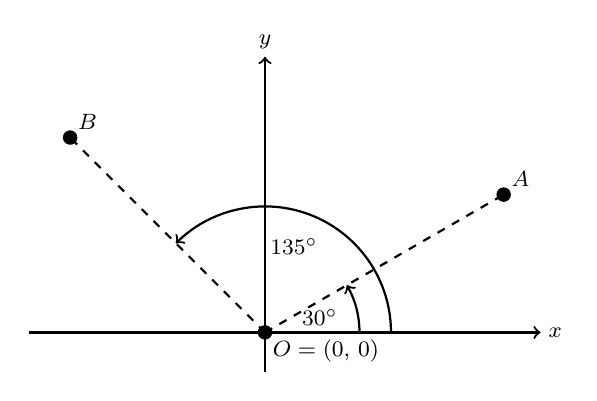
\begin{tikzpicture}[%%
  axisStyle/.style={->,thick},%%
  dashStyle/.style={-,thick,dashed},%%
  lineStyle/.style={-,thick},%%
  nodeStyle/.style={draw,inner sep=1.7pt,circle,fill=black,black}%%
]
%%
%%
\pgfmathsetmacro{\radius}{3.5}
\pgfmathsetmacro{\xa}{3.03108891324554}
\pgfmathsetmacro{\xhigh}{3.5}
\pgfmathsetmacro{\xlow}{-3}
\pgfmathsetmacro{\yb}{1.75000000000000}
\pgfmathsetmacro{\yhigh}{\xhigh}
\pgfmathsetmacro{\ylow}{-0.5}
%% The Cartesian coordinate system.
\coordinate (origin) at (0,0);
\coordinate (xend) at (\xhigh,0);
\coordinate (xstart) at (\xlow,0);
\coordinate (yend) at (0,\yhigh);
\coordinate (ystart) at (0,\ylow);
%% The generic angle.
\coordinate (point) at (\xa,\yb);
\coordinate (pointReflection) at (-2.47487373415292,2.47487373415292);
\coordinate (xyRadius) at (\radius,0);
%%
%%
%% Draw two points in the Cartesian coordinate system.
\footnotesize
\cartesianCoordinate
\genericPoint
\end{tikzpicture}

\end{document}
